\subsection{Results}
\label{sec:res}
In this section we show, for each implemented model, the achieved results and we compare them with the expected ones. We also show a comparison with the two models \textbf{(M1)} and \textbf{(M2)} on the \textbf{CUP} dataset.

For each tested model, we consider the achieved gradient norm and the score in terms of \textit{MSE} as performance metrics. For all the models based on a NN implementation, we imposed a different stopping condition for the two datasets, in particular:
\begin{itemize}
    \item \textbf{MONK}: stopping condition only based on the norm of the gradient, without selecting a particular amount of epochs;
    \item \textbf{CUP}: stopping condition based also on the number of epochs, this was due to the fact that a given accuracy on the norm of the gradient can't be reached by all the used models.
\end{itemize}

\subsubsection{MONK}
In this section we show the comparison of the different models over the three \textbf{MONK} datasets. In particular we compare the achieved losses and gradient, considering the number of epochs and the amount of time necessary to achieve the desired precision.

\begin{figure}[H]
	\centering
	\begin{subfigure}{.45\textwidth}
	    \centering
	    \subcaptionbox{}{%
            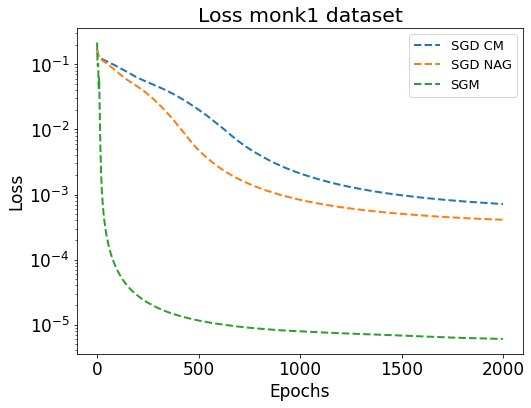
\includegraphics[width=\linewidth]{res/loss_monk1_ep.png}\hspace*{2.5em}%
        }
	\end{subfigure}
	\begin{subfigure}{.45\textwidth}
	    \centering
	    \subcaptionbox{}{%
            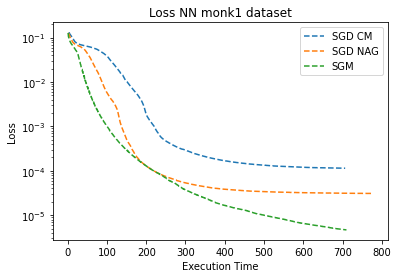
\includegraphics[width=\linewidth]{res/loss_monk1_time.png}\hspace*{2.5em}%
        }
	\end{subfigure}
    \par\bigskip % force a bit of vertical whitespace
	\begin{subfigure}{.45\textwidth}
	    \centering
	    \subcaptionbox{}{%
            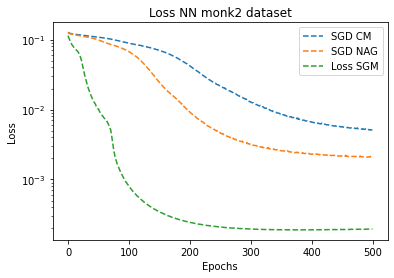
\includegraphics[width=\linewidth]{res/loss_monk2_ep.png}\hspace*{2.5em}%
        }
	\end{subfigure}
	\begin{subfigure}{.45\textwidth}
	    \centering
	    \subcaptionbox{}{%
            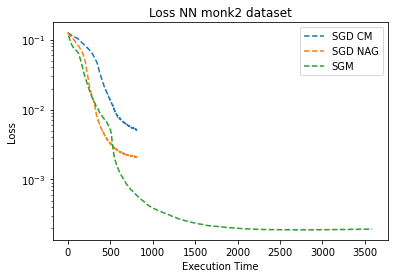
\includegraphics[width=\linewidth]{res/loss_monk2_time.png}\hspace*{2.5em}%
        }
	\end{subfigure}
	\par\bigskip % force a bit of vertical whitespace
	\begin{subfigure}{.45\textwidth}
	    \centering
	    \subcaptionbox{}{%
            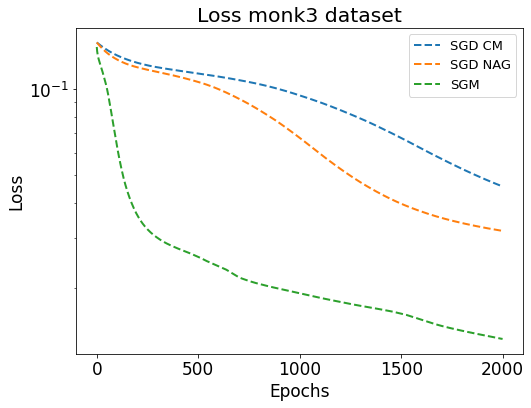
\includegraphics[width=\linewidth]{res/loss_monk3_ep.png}\hspace*{2.5em}%
        }
	\end{subfigure}
	\begin{subfigure}{.45\textwidth}
	    \centering
	    \subcaptionbox{}{%
            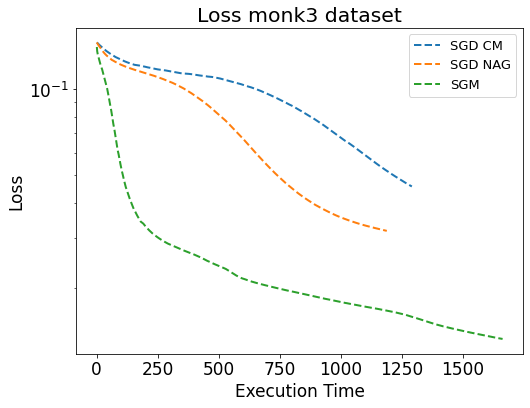
\includegraphics[width=\linewidth]{res/loss_monk3_time.png}\hspace*{2.5em}%
        }
	\end{subfigure}
	\caption{Comparison between the three tested models \texttt{SGD} (both with \textit{CM} and \textit{NAG}) and \texttt{SGM}. On each row we show the comparison on a different \textbf{MONK} dataset and the two columns represent, from left to right, the loss w.r.t.\ the number of epochs and the required time in milliseconds.}
	\label{fig:monk_loss}
\end{figure}

\begin{figure}[H]
	\centering
	\begin{subfigure}{.4\textwidth}
	    \centering
	    \subcaptionbox{}{%
            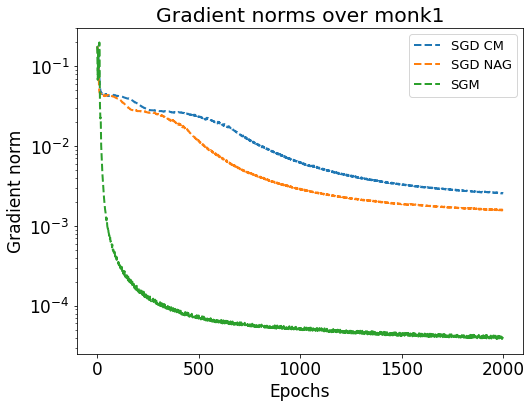
\includegraphics[width=\linewidth]{res/grad_monk1.png}\hspace*{2.5em}%
        }
	\end{subfigure}
	\begin{subfigure}{.4\textwidth}
	    \centering
	    \subcaptionbox{}{%
            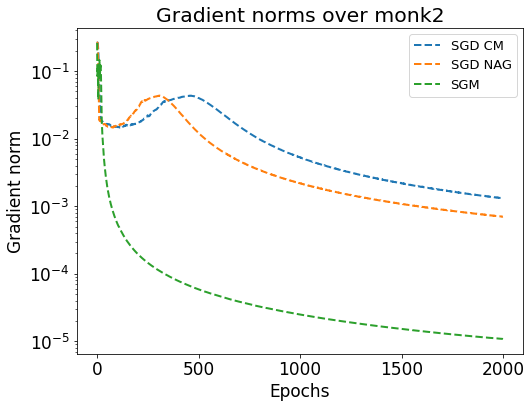
\includegraphics[width=\linewidth]{res/grad_monk2.png}\hspace*{2.5em}%
        }
	\end{subfigure}
	\begin{subfigure}{.45\textwidth}
        \centering
	    \subcaptionbox{}{%
            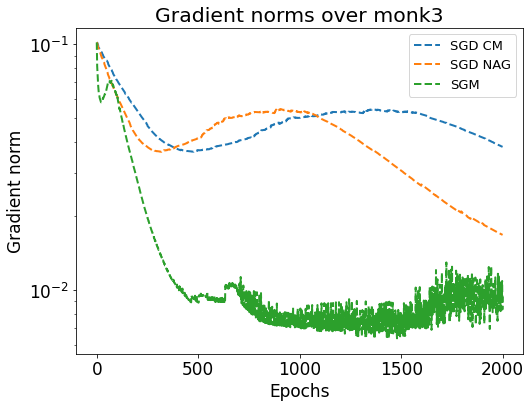
\includegraphics[width=\linewidth]{res/grad_monk3.png}\hspace*{2.5em}%
        }
	\end{subfigure}
	
	\caption{Gradient norm comparison over the three \textbf{MONK} datasets for the three tested models.}
	\label{fig:monk_grad}
\end{figure}

\begin{table}[H]
    \begin{center}
    \begin{adjustwidth}{0.cm}{}
    \begin{center}
    \resizebox{0.9\textwidth}{!}{%
    \begin{tabular}{|P{2.cm}||c|c|c|c|c|c|c|c|}
         \hline
         \textbf{Task} & \textbf{optimizer} & \textbf{batch\_size} & $\boldsymbol{\epsilon}$ & $\boldsymbol{\mu}$ & $\boldsymbol{\lambda}$ & \textbf{sizes} & $\nabla f_*$ & $f_*$ \\ [0.5ex] 
         \hline\hline
         MONK1 & CM & 32 & 0.1 & 0.9 & 0.1 & 5 & \num{1.271e-2} & \num{1.145e-4}\\
         \hline
         MONK1 & NAG & 32 & 0.1 & 0.9 & 0.01] & 5 & \num{6.801e-3} & \num{3.088e-5}\\
         \hline
         MONK1 & SGM & None & 0.1 & - & 0.01 & 5 & \num{8.020e-4} & \num{4.662e-6}\\
         \hline\hline
         MONK2 & CM & 32 & 0.1 & 0.5 & 0.01 & 3 & \num{5.328e-2} & \num{5.079e-3}\\
         \hline
         MONK2 & NAG & 32 & 0.1 & 0.5 & 0.01 & 3 & \num{4.719e-2} & \num{2.090e-3}\\
         \hline
         MONK2 & SGM & 10 & 0.1 & - & 0.01 & 3 & \num{1.935e-2} & \num{1.898e-4}\\
         \hline\hline
         MONK3 & CM & 10 & 0.1 & 0.9 & 0.01 & 5 & \num{1.635e-2} & \num{8.945e-3}\\
         \hline
         MONK3 & NAG & 10 & 0.1 & 0.9 & 0.01 & 5 & \num{7.106e-3} & \num{3.391e-3}\\
         \hline
         MONK3 & SGM & None & 0.1 & - & 0.01 & 5 & \num{2.449e-3} & \num{6.921e-4}\\
         \hline
    \end{tabular}}
    \end{center}
    \end{adjustwidth}
    \subcaption{Test results over \textbf{MONK} datasets. Models chosen via gridsearch as shown in \S\ref{sec:res}}
    \label{tab:res_MONK}
    \end{center}
    \hspace{2em}
    \begin{center}
    \resizebox{0.6\textwidth}{!}{%
    \begin{tabular}{|P{2.cm}||c|c|c|c|c|}
         \hline
         \textbf{Task} & \textbf{optimizer} & \textbf{epochs} & \textbf{total} & \textbf{BP} & \textbf{EP} \\ [0.5ex] 
         \hline\hline
         MONK1 & CM & 500 & 601.93 & 0.078 & 1.203 \\
         \hline
         MONK1 & NAG & 500 & 497.99 & 0.061 & 0.995 \\
         \hline
         MONK1 & SGM & 1000 & 604.02 & 0.228 & 0.604 \\
         \hline\hline
         MONK2 & CM & 500 & 693.86 & 0.062 & 1.387 \\
         \hline
         MONK2 & NAG & 500 & 924.36 & 0.078 & 1.848 \\
         \hline
         MONK2 & SGM & 500 & 3496.17 & 0.210 & 6.992 \\
         \hline\hline
         MONK3 & CM & 500 & 1360.03 & 0.059 & 2.720 \\
         \hline
         MONK3 & NAG & 500 & 1772.94 & 0.074 & 3.545 \\
         \hline
         MONK3 & SGM & 1000 & 751.25 & 0.277 & 0.751 \\
         \hline
    \end{tabular}}
    \subcaption{Execution statistics relative to the models used for testing in table \ref{tab:res_MONK}.}
    \label{tab:gridSGM}
    \end{center}
    \caption{Execution results and performances for the models selected via gridsearch.}
    \label{tab:stat_MONK}
\end{table}

In \hyperref[tab:res_MONK]{\textbf{Table \ref{tab:res_MONK}}} we clearly see an increased cost for the \textit{backpropagation} computation for the \texttt{SGM} model. This was due to the fact that this model requires to update the stepsize at the end of each iteration in order to converge to a solution. This inevitably introduces a bottleneck in the computation of the backpropagation algorithm compared to the \texttt{SGD} model.

\subsubsection{CUP}
In this section we show the comparison of different models over the CUP dataset. We show the achieved loss and gradient norms for all the tested models.
\begin{figure}[H]
	\centering
	\begin{subfigure}{.4\textwidth}
	    \centering
	    \subcaptionbox{}{%
            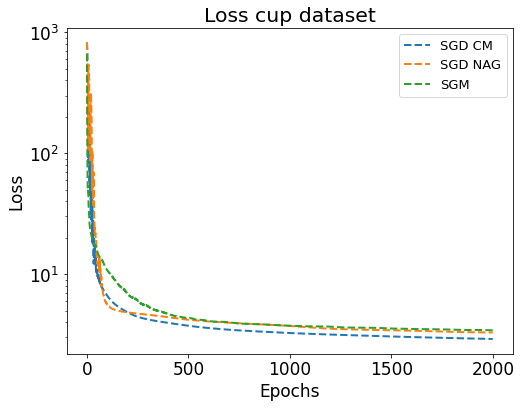
\includegraphics[width=\linewidth]{res/loss_cup_ep.png}\hspace*{2.5em}%
        }
	\end{subfigure}
	\begin{subfigure}{.4\textwidth}
	    \centering
	    \subcaptionbox{}{%
            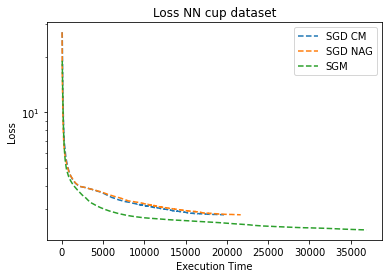
\includegraphics[width=\linewidth]{res/loss_cup_time.png}\hspace*{2.5em}%
        }
	\end{subfigure}
    
	\caption{Comparison between the three tested models \texttt{SGD} (both with \textit{CM} and \textit{NAG}) and \texttt{SGM} over the CUP dataset. Image \textbf{(a)} and \textbf{(b)} show, respectively, the loss w.r.t.\ the number of epochs and the required time in milliseconds.}
	\label{fig:cup_loss}
\end{figure}

\begin{figure}[H]
	\centering
    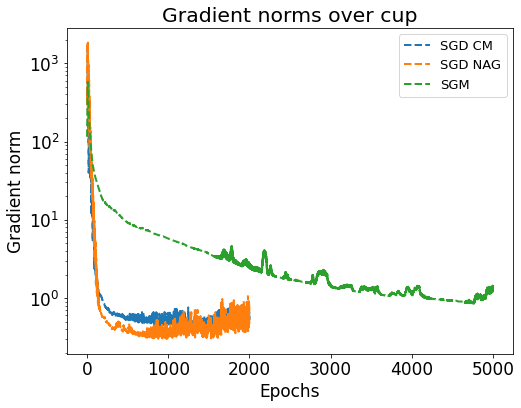
\includegraphics[width=0.4\linewidth]{res/grad_cup.png}\hspace*{2.5em}%
	
	\caption{Gradient norm comparison over the \textbf{CUP} dataset for the three tested models.}
	\label{fig:cup_grad}
\end{figure}

\begin{table}[H]
    \begin{center}
    \begin{adjustwidth}{0.cm}{}
    \begin{center}
    \resizebox{0.9\textwidth}{!}{%
    \begin{tabular}{|P{2.cm}||c|c|c|c|c|c|c|c|}
         \hline
         \textbf{Task} & \textbf{optimizer} & \textbf{batch\_size} & $\boldsymbol{\epsilon}$ & $\boldsymbol{\mu}$ & $\boldsymbol{\lambda}$ & \textbf{sizes} & $\nabla f_*$ & $f_*$ \\ [0.5ex] 
         \hline\hline
         CUP & CM & 32 & 0.1 & 0.9 & 0.1 & 5 & \num{1.271e-2} & \num{1.145e-4}\\
         \hline
         CUP & NAG & 32 & 0.1 & 0.9 & 0.01] & 5 & \num{6.801e-3} & \num{3.088e-5}\\
         \hline
         CUP & SGM & None & 0.1 & - & 0.01 & 5 & \num{8.020e-4} & \num{4.662e-6}\\
         \hline
    \end{tabular}}
    \end{center}
    \end{adjustwidth}
    \subcaption{Test results over \textbf{CUP} dataset. Models chosen via gridsearch as shown in \S\ref{sec:res}}
    \label{tab:res_CUP}
    \end{center}
    \hspace{2em}
    \begin{center}
    \resizebox{0.65\textwidth}{!}{%
    \begin{tabular}{|P{2.cm}||c|c|c|c|c|}
         \hline
         \textbf{Task} & \textbf{optimizer} & \textbf{iterations} & \textbf{total} & \textbf{BP} & \textbf{EP} \\ [0.5ex] 
         \hline\hline
         CUP & CM & 1000 & 20059 & 0.187 & 20.059 \\
         \hline
         CUP & NAG & 1000 & 20061 & 0.182 & 20.061 \\
         \hline
         CUP & SGM & 1000 & 33282 & 0.526 & 33.282 \\
         \hline
    \end{tabular}}
    \subcaption{Execution statistics relative to the models used for testing in table \ref{tab:res_MONK}.}
    \label{tab:gridSGM}
    \end{center}
    \caption{Execution results and performances for the models selected via gridsearch.}
    \label{tab:stat_CUP}
\end{table}